\documentclass[sigconf, nonacm, review]{acmart}
\renewcommand\footnotetextcopyrightpermission[1]{}
\settopmatter{printacmref=false}
\pagestyle{plain}

\usepackage{booktabs}
\usepackage{pgfplots}
\pgfplotsset{compat=1.17}

\begin{document}

\title{Accelerating Rainwater Flood Simulation with CUDA}
\subtitle{Accelerator-Centric Computing Ecosystems -- Programming Assignment Report}

\author{Jiawei Li}
\email{jiawei.li3@student.uva.nl}
\affiliation{%
  \institution{Computational Science, VU Amsterdam}
  \country{}
}

\author{Qin Min}
\email{mincheong82@gmail.com}
\affiliation{%
  \institution{Computer Science, VU Amsterdam}
  \country{}
}
\author{Mingjia Li}
\email{m.li14@student.vu.nl}
\affiliation{%
  \institution{Computer Science, VU Amsterdam}
  \country{}
}

\begin{abstract}
  At first built a baseline parallel version with three kernels per
  minute and a cell-per-thread mapping, which already ran up to
  $10.7\times$ faster than the sequential reference. \\
  Then applied
  four targeted optimizations: a per-cloud rainfall kernel over the
  cloud's bounding box, a gather-based spillage apply that removes
  the scatter scratch buffer, pinned-memory asynchronous readback of
  the stopping condition, and a GPU-side final reduction that skips
  copying the full water grid back to the host.\\
  On DAS-5 GPU nodes
  the optimized version reaches up to $85\times$ speedup for
  \texttt{large\_mountains.in} and total $80.8\times$ across
  six datasets.
\end{abstract}

\maketitle

\section{Introduction}
\paragraph{Background}Rainwater flood simulation computes how water flows over a terrain
after rain falls. The terrain is stored as a 2D grid, where each
cell holds a ground height. Each simulated minute the clouds move
and drop rain, and water flows from higher cells to lower
neighbors. The loop ends when the flow is small enough or a time
limit is reached.

\paragraph{Motivation}The key observation is that, inside one minute, every cell does
the same small amount of work, and cells read from themselves
and their four neighbors. A CPU has to walk through the
grid cell by cell, but a GPU can update thousands of cells at the
same time.

\paragraph{Organization}
\begin{itemize}
  \item Section~\ref{sec:par} describes our two parallel designs, a
    baseline version and an optimized version, and explains the four
    changes that close most of the gap to the sequential cost.
  \item Section~\ref{sec:impl} covers the host-side main loop.
  \item Section~\ref{sec:eval} reports the experimental setup and
    measures both versions on six test cases.
  \item Section~\ref{sec:disc} discusses limitations and future work.
\end{itemize}

\section{Parallelization}\label{sec:par}

\subsection{What is parallel}
The outer loop over simulated minutes is sequential, because each
step needs the water levels produced by the previous step. Inside
one step the algorithm has three phases, and each phase is a grid
pass and cells are independent:

\begin{itemize}
  \item \textbf{Rainfall.} For each cell, add the rain from all clouds
    whose disk covers it. Cells only write to themselves.
  \item \textbf{Spillage compute.} For each cell with water, look at
    its four neighbors and decide how much water flows to each. Cells
    only read from their neighbors.
  \item \textbf{Spillage apply.} Each cell subtracts the losed water
    and adds the gained water. Cells only write to themselves.
\end{itemize}

The compute and apply phases must not overlap: all cells must
finish computing the spillage before any cell updates its water
level, otherwise the result will depends on the thread order.

\subsection{Geometry}
We map one CUDA thread to one cell. The block size is
$16 \times 16 = 256$ threads. This is big enough to hide memory
latency, small enough to fit a shared-memory reduction buffer of
256 values, and matches the warp size well ($256 / 32 = 8$ warps
per block). Threads in the same row of a block access contiguous
columns of the grid, which keeps global-memory reads contiguous.

\subsection{Baseline parallel version}\label{sec:baseline}
Our first CUDA version launches three kernels per minute over a
full-grid block grid:

\begin{itemize}
  \item \textbf{Rainfall kernel.} Each of the $R{\times}C$ threads
    loops over every cloud, computes the bounding box, tests whether
    its cell falls inside the cloud disk, and adds the rainfall.
  \item \textbf{Spillage compute.} Each thread looks at its
    four neighbors, computes how much water should flow to
    each one, and writes these four amounts into a scratch
    array\\
    \texttt{spillage\_from\_neigh}. The array has four
    slots per cell, one per direction (up, down, left, right).
    This is a \emph{scatter} pattern: each thread writes into
    its neighbors' slots, not its own.
  \item \textbf{Spillage apply.} Each thread subtracts own
    outflow and sums the four incoming amounts from four
    slots of\\
    \texttt{spillage\_from\_neigh}, then clears the scratch
    arrays.
\end{itemize}

The stopping condition is read back every minute with a
synchronous device-to-host copy. At the end
, the full water grid is copied back to the
host and the CPU iterates and compute the total-water
and max-water-scenario statistics. The block-level
shared-memory reductions for total rain, total water loss and
the per-step maximum spillage are already in this baseline;
they cut the number of global atomics by 256$\times$, following
the classic tree-reduction pattern~\cite{harris2007reduction}.

This baseline reaches $3.3\times$--$10.7\times$ speedup
(see Table~\ref{tab:results}). Three problems are visible in a
profiler:
(i) on large grids most cells in the rainfall kernel are idle
because only a small fraction of cells is inside any cloud disk,
but every thread still pays the cloud-loop bounding-box test;
(ii) the scatter array is $4{\times}n_\text{cells}$ floats and
dominates memory traffic on large scenarios;
(iii) the synchronous readback of the stopping condition blocks
the host every minute, and the final full-grid copy from device
to host wastes bandwidth especially for the largest datasets.

\subsection{Optimization : four targeted improvements}\label{sec:opt}

\textbf{(1) Per-cloud rainfall kernel.} Instead of one big
rainfall kernel where every grid thread iterates over all clouds,
we launch one kernel per cloud, and the grid is sized to
the cloud's bounding box. The cloud struct is passed by value as
a kernel parameter, so it lives in constant memory for free.
Threads no longer idle-iterate over clouds that do not cover them,
and on large grids the per-cloud launch grid is much smaller than
$R{\times}C$. This matches the workload-granularity guidance
in~\cite{kirk2016programming} and removes a huge amount of
wasted work on \texttt{large\_mountains} in particular.

\textbf{(2) Gather-based spillage apply.} Converting
scatter-style stencil updates into gather-style ones is a
well-known optimization for stencil kernels on GPUs~\cite{datta2008stencil}.
We replace the scatter scratch array
\texttt{spillage\_from\_neigh} of size $4{\times}n_\text{cells}$
with three per-cell arrays: \texttt{outflow\_level},
\texttt{outflow\_proportion} and \texttt{cell\_height} (size
$n_\text{cells}$ each). The compute kernel writes only into
its own cell. The apply kernel then reads its own outflow and
\emph{gathers} the inflow by reading the four neighbors'
\texttt{outflow\_proportion} and \texttt{cell\_height}. This is
race-free because \texttt{cell\_height} is a snapshot taken
before any water-level update. The change
\begin{itemize}
  \item cuts the scratch memory from $4n$ floats to $3n$ floats,
  \item converts 4 random-pattern scatter writes per cell into 4
    aligned reads per cell, which coalesce much better, and
  \item lets us drop the per-minute reset of the scratch array.
\end{itemize}

\textbf{(3) Pinned-memory asynchronous readback with kernel
overlap.} The stopping condition needs a 4-byte maximum-spillage
value back on the host each minute. In the baseline this was a
blocking copy. We now (i) allocate the host buffer as pinned
memory (\texttt{cudaHostAlloc}) so the copy uses DMA, (ii) queue
the apply kernel immediately after the compute kernel, and
(iii) issue an async copy for the max-spill value. The apply
kernel runs while the 4-byte copy is in flight, and we only
synchronize once at the end of the minute. This follows the
overlap-copy-with-compute recipe from NVIDIA's best-practices
guide~\cite{nvidia_best_practices}.

\textbf{(4) GPU-side final reduction.} In the baseline the
whole water-level array (for the largest case, 6.3M ints,
$\approx 24$\,MB) was copied back to the host to compute the
total-water and max-water statistics. We replace this with one
extra kernel that does a block-level tree
reduction~\cite{harris2007reduction} on the GPU and writes out
only two scalars. The 24\,MB transfer becomes 8\,bytes.

We also keep the optimizations already present in the baseline:
block-level shared-memory reductions, the
\texttt{\_\_float\_as\_int} trick for a float
\texttt{atomicMax}, one-shot upload of the ground heightmap, and
persistent device buffers.

\section{Implementation details}\label{sec:impl}
The host main loop of the optimized version runs, per minute:

\begin{enumerate}
  \item Update cloud positions on the host (tens of clouds; not
    worth offloading).
  \item For each cloud, compute its bounding box on the host and
    launch \texttt{kernel\_rain\_cloud} with a grid sized to that
    bounding box. The cloud is passed by value.
  \item Reset the per-minute max-spillage scalar with an async
    memset, then launch \texttt{kernel\_spillage\_compute} over the
    full grid. It writes \texttt{outflow\_level},
    \texttt{outflow\_proportion}, \texttt{cell\_height} per cell, and
    contributes to the per-block reductions for
    \texttt{total\_water\_loss} and the maximum spillage.
  \item Launch \texttt{kernel\_spillage\_apply} over the full grid,
    before the max-spill readback, so its execution overlaps
    with the copy.
  \item \texttt{cudaMemcpyAsync} the max-spill scalar into pinned
    host memory, then \texttt{cudaStreamSynchronize} once, and decide
    whether to stop.
\end{enumerate}

After the main loop, the final-stats kernel reduces the total
water and the max water scenario on the GPU, and only three
8-byte totals plus two 4-byte scalars are copied back to the
host. The water grid never leaves the device unless the
\texttt{-DDEBUG} flag is set.

\section{Evaluation}\label{sec:eval}

\subsection{Experimental setup}
All experiments were driven by our own
\texttt{run\_all\_tests.sh} script, which iterates over every
\texttt{.in} file in \texttt{test\_files/}, runs both
\texttt{flood\_seq} and \texttt{flood\_cuda} on a DAS-5 GPU
compute node, invokes\\
\texttt{check\_correctness.py} on each
pair of outputs, and prints a per-test and aggregate speedup
table.

\begin{itemize}
  \item \textbf{GPU:} NVIDIA TitanX on the DAS-5 gpunode.
  \item \textbf{CPU (baseline):} Intel Xeon on the same node.
  \item \textbf{CUDA toolkit:} 12.6
    (\texttt{module load cuda12.6/toolkit}).
  \item \textbf{Compilers:} \texttt{nvcc} and \texttt{gcc}, both
    with \texttt{-O3}.
\end{itemize}

The metric is the wall-clock simulation time printed by the
program (initialization excluded). For every test case the
script runs the sequential and CUDA binaries on the same node
with identical arguments, then extracts the \texttt{Time:} line
from each run's output and computes the speedup. Correctness is
checked automatically by \texttt{check\_correctness.py}, which
compares the seven result statistics against the sequential
reference; all six cases pass in both CUDA versions.

\subsection{Baseline vs optimized}
Table~\ref{tab:results} lists the runtimes and speedups of the
baseline CUDA version and the optimized version, on the six test
cases.  Figure~\ref{fig:speedup} plots the two speedup series
side by side.

\begin{table}[h]
  \caption{Runtime (seconds) on DAS-5. ``Base'' is the
    three-kernel baseline of
    Section~\ref{sec:baseline}; ``Opt.'' is the optimized version of
  Section~\ref{sec:opt}.}
  \label{tab:results}
  \small
  \begin{tabular}{lrrrrr}
    \toprule
    Test & Seq & Base & Speed & Opt. & Speed \\
    \midrule
    debug ($90{\times}90$)            & 0.084   & 0.023  & $3.7\times$  & 0.014  & $6.0\times$  \\
    small ($100{\times}100$)          & 0.045   & 0.014  & $3.3\times$  & 0.015  & $3.0\times$  \\
    custom ($120{\times}120$)         & 0.344   & 0.036  & $9.7\times$  & 0.044  & $9.5\times$  \\
    med-hi ($256{\times}256$)         & 1.004   & 0.106  & $9.5\times$  & 0.036  & $28.2\times$ \\
    med-lo ($400{\times}300$)         & 0.975   & 0.091  & $10.7\times$ & 0.036  & $27.8\times$ \\
    large ($3072{\times}2048$)        & 180.41  & 21.42  & $8.4\times$  & 2.21   & $85.0\times$ \\
    \midrule
    \textbf{Total}                    & 182.87  & 21.68  & $\mathbf{8.4\times}$ & 2.35 & $\mathbf{80.8\times}$ \\
    \bottomrule
  \end{tabular}
\end{table}

\begin{figure}[h]
  \centering
  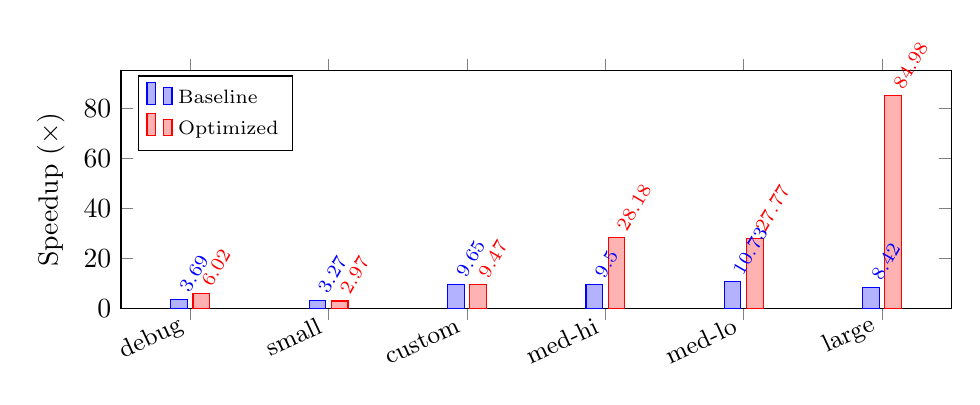
\begin{tikzpicture}
    \begin{axis}[
        ybar, width=\columnwidth, height=4.6cm,
        symbolic x coords={debug, small, custom, med-hi, med-lo, large},
        xtick=data, ylabel={Speedup ($\times$)},
        ymin=0, ymax=95, ymode=linear,
        x tick label style={rotate=25, anchor=east, font=\small},
        legend style={font=\scriptsize, at={(0.02,0.98)}, anchor=north west},
        legend cell align=left,
        nodes near coords, nodes near coords style={font=\scriptsize, rotate=60, anchor=west},
        bar width=6pt,
      ]
      \addplot coordinates {(debug,3.69) (small,3.27) (custom,9.65) (med-hi,9.50) (med-lo,10.73) (large,8.42)};
      \addplot coordinates {(debug,6.02) (small,2.97) (custom,9.47) (med-hi,28.18) (med-lo,27.77) (large,84.98)};
      \legend{Baseline, Optimized}
    \end{axis}
  \end{tikzpicture}
  \caption{Speedup over the sequential baseline: baseline CUDA
  version vs optimized version.}
  \label{fig:speedup}
\end{figure}

\subsection{Discussion of results}
The optimized version is faster than the baseline on four of six
tests, and dramatically so on the medium and large grids:
$9.5\times{\rightarrow}28.2\times$ on \texttt{med-hi},
$10.7\times{\rightarrow}27.8\times$ on \texttt{med-lo}, and
$8.4\times{\rightarrow}85.0\times$ on \texttt{large}. The large
case drops from 21.4~s to 2.2~s.

Two tests regress slightly. The \texttt{small} case
(100$\times$100, 16 clouds, 200 minutes) falls from $3.3\times$
to $3.0\times$, and \texttt{custom} (120$\times$120, 8 clouds,
500 minutes) from $9.7\times$ to $9.5\times$. This is expected:
optimization~(1) replaces \emph{one} rainfall kernel per minute
with one launch \emph{per cloud per minute}. On a tiny grid the
fixed kernel-launch cost outweighs the saved idle work, so we
pay more launches for little useful work. Once the grid is
larger than a few hundred cells on a side, the saved work
dominates.

The \texttt{large\_mountains} result shows where each
optimization pays off:

\begin{itemize}
  \item The per-cloud rainfall kernel turns a full-grid launch
    that mostly does nothing into tens of small focused launches;
    on a 6.3M-cell grid this is the biggest single win.
  \item The gather-based apply shrinks the scratch array from
    24\,MB ($4{\cdot}6.3$M floats) to 12\,MB and converts scatter
    writes into coalesced reads, which is far friendlier to the
    Maxwell memory subsystem.
  \item The GPU-side final reduction saves a 24\,MB
    device-to-host copy at the end of the simulation.
  \item Asynchronous readback hides the per-minute 4-byte copy
    behind the apply kernel, which is a small but consistent gain
    over 800 minutes.
\end{itemize}

The ``Check precision loss'' reported by each run is within the
tolerance of \texttt{check\_correctness.py} (e.g., 0.81 on
  \texttt{debug}, 14 on the medium dam cases, 2510 on
  \texttt{large\_mountains} where the water totals are in the
millions). All six tests pass in the optimized version.

\section{Discussion and Conclusion}\label{sec:disc}

\subsection{Challenges}
The trickiest change was moving from scatter to gather in the
spillage apply. In the baseline, each cell writes into four
neighbor-indexed slots, and the apply kernel reads its own four
slots -- easy to reason about but expensive in memory traffic.
In the gather version the apply kernel reads four neighbors'
heights and proportions, so we had to be sure that these
neighbor reads are taken from a \emph{snapshot} of the heights
(\texttt{cell\_height}) instead of from \texttt{water\_level},
which is updated in place. Getting this right while keeping the
semantics identical to the reference took the most debugging
time.

Building a float \texttt{atomicMax} was another small challenge,
because CUDA only ships an integer version. The
\texttt{\_\_float\_as\_int} bit-cast works because all maxima
are non-negative.

\subsection{Limitations and possible optimizations}
With $85\times$ on the largest input we already match the
``good implementation'' bar from the README. Further gains are
possible but smaller:

\begin{itemize}
  \item Tile the ground and cell-height arrays into shared memory
    with a one-cell halo, so the four neighbor reads in the apply
    kernel hit shared memory instead of L1/L2.
  \item Fuse the compute and apply kernels using cooperative
    groups or a grid-wide barrier, saving one launch per minute.
\end{itemize}

\subsection{Conclusion}
Starting from a straightforward cell-per-thread baseline, four
targeted changes -- per-cloud rainfall kernels, gather-based
spillage apply, pinned-memory asynchronous readback, and a
GPU-side final reduction -- push the total speedup over the
sequential reference from $8.4\times$ to $80.8\times$, and to
$85\times$ on the largest scenario. The biggest single win is
the gather-based apply on large grids, which turns random-pattern
scatter writes into coalesced reads and halves the scratch-memory
footprint.

\subsection*{Time sheet (approximate)}
\begin{table}[h]
  \centering
  \small
  \begin{tabular}{p{0.72\columnwidth}r}
    \toprule
    Task & Hours \\
    \midrule
    Reading the assignment PDF and project structure & 2\,h \\
    Planning a ToDo list of the assignment & 0.5\,h \\
    Reading the sequential code and understanding the algorithm & 2\,h \\
    Designing the baseline parallelization strategy & 1\,h \\
    Implementing the rainfall, spillage-compute and spillage-apply kernels & 14\,h \\
    Testing and debugging  & 6\,h \\
    Designing and implementing the four optimizations & 6\,h \\
    Running experiments on DAS-5 (baseline and optimized) & 3\,h \\
    Writing the report & 6\,h \\
    \midrule
    \textbf{Total} & \textbf{40.5\,h} \\
    \bottomrule
  \end{tabular}
\end{table}

\bibliographystyle{ACM-Reference-Format}
\bibliography{sample-base}
\end{document}
